%%%%%%%%%%%%%%%%%%%%%%%%%%%%%%%%%%%%%%%%%%%%%%%%%%%%%%%%%%%%%%%%%%%%%
% LaTeX Template: Project Titlepage Modified (v 0.1) by rcx
%
% Original Source: http://www.howtotex.com
% Date: February 2014
% 
% This is a title page template which be used for articles & reports.
% 
% This is the modified version of the original Latex template from
% aforementioned website.
% 
%%%%%%%%%%%%%%%%%%%%%%%%%%%%%%%%%%%%%%%%%%%%%%%%%%%%%%%%%%%%%%%%%%%%%%

\documentclass[12pt]{article}
\usepackage[a4paper]{geometry}
\usepackage[myheadings]{fullpage}
\usepackage{fancyhdr}
\usepackage{lastpage}
\usepackage{graphicx, wrapfig, subcaption, setspace, booktabs}
\usepackage[T1]{fontenc}
\usepackage[font=small, labelfont=bf]{caption}
\usepackage{fourier}
\usepackage[protrusion=true, expansion=true]{microtype}
\usepackage[english]{babel}
\usepackage{sectsty}
\usepackage{url, lipsum}
\usepackage{tabularx}

\newcommand\boldblue[1]{\textcolor{blue}{\textbf{#1}}}
\newcommand{\HRule}[1]{\rule{\linewidth}{#1}}
\onehalfspacing
\setcounter{tocdepth}{5}
\setcounter{secnumdepth}{5}

%-------------------------------------------------------------------------------
% HEADER & FOOTER
%-------------------------------------------------------------------------------
\pagestyle{fancy}
\fancyhf{}
\setlength\headheight{15pt}
\fancyhead[L]{CHARM}
\fancyhead[R]{Carleton University}
\fancyfoot[R]{Page \thepage\ of \pageref{LastPage}}
%-------------------------------------------------------------------------------
% TITLE PAGE
%-------------------------------------------------------------------------------

\begin{document}
\bibliographystyle{ieeetr}

\title{ \normalsize \textsc{}
		\\ [2.0cm]
		\HRule{0.5pt} \\
		\LARGE \textbf{{Carleton High Altitude Radiometer}}\\
		\large \textbf{{Project Proposal}}\\
		\large \textbf{{Canadian Stratospheric Balloon Experiment Design Challenge}}
		\HRule{2pt} \\ [0.5cm]
		\normalsize \today \vspace*{2\baselineskip}\\
		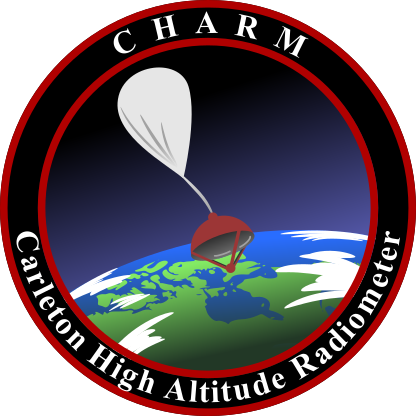
\includegraphics[scale=0.6]{Figures/CHARM.png}	\vspace*{2\baselineskip} \\
		\textsc{
		Jacob Booth \\
		David Bascelli \\
		}}
		
\date{}
	
\author{
		Carleton University \\
		}
	


\maketitle

\newpage

\tableofcontents
\newpage

\listoffigures
\newpage

\listoftables
\newpage

%-------------------------------------------------------------------------------
% Section title formatting
\sectionfont{\scshape}
%-------------------------------------------------------------------------------

%-------------------------------------------------------------------------------
% BODY
%-------------------------------------------------------------------------------

\section{Executive Summary}
Microwave remote sensing has been a common payload on earth observation satellites since the early days of space-flight. In as early as 1962, a radiometer on-board the Mariner 2 mission measured the surface temperature of Venus. 1968 Saw the first space-born earth observation radiometer on-board the  Cosmos 243 satellite, which measured atmospheric water vapour and global ice cover. Many different radiometer configurations can make a wide array of different geological, biological, and climate measurements. The CHARM project will design and manufacture a balloon mounted microwave radiometer for the purpose of measuring soil moisture content over a large area. Soil moisture measurements are crucial in predicting local weather conditions and monitoring climate change. Incorporating soil moisture measurements into weather and climate models allows for more accurate medium term weather forecasts and can also give clues about future droughts, crop yields, and water resource management. Currently, most radiometric data comes from space-born radiometers, such as those on the SMAP or SMOS satellites. To achieve high resolution and accuracy, these space-born radiometers utilize cryogenic components, complex phased array or synthetic aperture technologies, and require large and very directional antennas. Our belief is that measurements of similar similar quality could be performed from a high altitude balloon at significantly reduced cost. 

\newpage

\section{Proposal}
\subsection{Scientific Objectives}

Our scientific objective is to make low cost measurements of soil moisture content using a balloon born passive microwave radiometer. The payload will take wide-band measurements of the noise equivalent temperature of the ground and determine soil moisture content through a modification of the zeroth order radiative transfer model (ZRT Model). A basic dielectric model will be used to solve for volumetric moisture content. \cite{ulaby_fung_moore_1986} A NADIR pointing antenna will extend from the pelican case to take measurements of the background microwave emissions coming from the ground. The radiometer will be of the Dicke type, which compares measurements to a known noise source to eliminate the effect of varying gain due to extreme temperatures. A 9-axis inertial measurement unit (IMU) will measure linear acceleration, angular rates, and magnetic field strength to determine the attitude of the payload. GPS data will be saved to track the location of the payload as it passes over the earth. With the attitude and GPS data, a map of soil moisture content under the payloads flight path will be able to be made. 

A Balloon born microwave radiometer to measure soil moisture was selected for several reasons. First, soil moisture content was chosen to be measured because of its importance to weather and climate monitoring.\cite{Pan2001} Soil moisture measurements are useful in many different circumstances. Climate models, weather predictions, crop yield estimation and water resource management systems all benifit from accurate and up to date measurements of ground moisture content. Soil moisture measurements have also proved useful in predicting wildfires.\cite{chaparro_piles_vall-llossera_2016,krueger_ochsner_quiring_engle_carlson_twidwell_fuhlendorf_2017} Second, measuring soil moisture content from radiometers is reasonably common and a significant amount of literature exists on the topic. Most literature either concerns satellite born radiometers, aircraft born radiometers, or static ground based radiometers. \cite{Hanington,Kerr2001,ulaby_fung_moore_1986,Friesen2008,Schmugge1994} By exploring the possibility of balloon based radiometers and by attempting more advanced soil moisture estimation techniques, we can achieve a degree of novelty while still having a wealth of proven literature and designs to aid us. Third, balloon mounted radiometers have several advantages to static, aircraft mounted, and satellite radiometers. Due to the balloon's proximity to the ground compared to low earth orbit, balloon born radiometers can achieve greater resolution with smaller and less directional antennas. Balloon radiometers can achieve much greater loiter times than aircraft born radiometers, although balloons are uncontrolled. Balloon born radiometers also have the advantage of being significantly cheaper to operate than aircraft or satellite mounted radiometers. A trade study was performed in table \ref{tab:vehicle_trade}, and it can be seen that balloon born radiometers offer a unique performance compromise at very low cost when compared to aircraft mounted or satellite based radiometers.

\begin{table}[!h]
	\centering
	\vspace{0.5cm}
	\renewcommand{\arraystretch}{1.3}
	\caption{Radiometer Vehicle Trade Study. }
	\label{tab:vehicle_trade}
	\begin{tabularx}{\textwidth}{llll}
		\toprule
						& Satellite & Aircraft & Balloon \\		
		\midrule
		Cost					&Very High&Moderate&Low \\ 
		Antenna Size 			&Large&Small&Small/Medium \\
		Resolution 				&Low Resolution&High Resolution&Medium Resolution \\ 
		Atmospheric Effects		&High&Low&Moderate \\ 
		Loiter Time				&N/A&Up to 6 hours&6 - 48 Hours \\ 
		Controllability			&Uncontrolled but predictable&Controlled&Uncontrolled 
	\end{tabularx}
\end{table}

Lastly, soil moisture retrieval from radiometric data is one of the simpler radiometer configurations to design and operate, allowing our team to gain experience with radiometer principals before attempting more advanced designs. Thus, a microwave radiometer was chosen as our balloon payload because of its many geoscientific applications, the wealth of literature and design aids, their suitability to the high altitude balloon environment, and because it allows us to gain experience with a relatively simple radiometer configuration.
 
\subsection{Experiment Design}

Passive microwave radiometers work by measuring the electromagnetic radiation emitted from the earth's surface in the microwave band. Liquid water content and water vapour is translucent to microwave frequencies, so an estimation of soil water content can be made by measuring the power of the emitted noise. By utilizing modern digital signal processing techniques, a wide-band power spectral density of the noise will be calculated. Using a radiative transfer model and potentially utilizing tertiary datasets, the power spectral density will be able to give a measurement of soil moisture content.

\subsubsection{Antenna Selection and Fabrication}
The design and construction of the antenna system presents many challenges, both in our radiometer and in space 
based systems. Antennas must be highly directional (have a high gain), which typically requires them to be quite large and heavy. In addition, lower frequencies require bigger antennas. In fact, earlier iterations of the design 
operated at a much lower frequency to make the electronics simpler, however it would not have been possible to fit
the antenna. Therefore, antenna sizing is the defining constraint on this system.\\

There are two solutions under consideration for the design of the antenna. A single large antenna, or an antenna 
array. Using an array of radiometers, we can create a synthetic aperture radiometer (SAR). With this solution we
would likely measure at 1.4 GHz, reducing hardware expense and complexity. This would involve precisely placing
four to eight antennas around the base of the gondola. The individual antennas would only be 10 cm long, and
weight very little. Coax cable would then need to be routed back to the experiment case. The use of SAR is common
in space based installations, as it is far lighter then having a large dish \cite{skou1989microwave}. 
However, the placement of many antennas, and the routing of many cables through the gonadal would be 
problematic. In addition the signal processing required to get meaningful data from a SAR is incredibly complex
and difficult, making this solution undesirably. It is mentioned in the event that the second solution does 
not work.\\

The second solution is to use a large horn antenna which sticks out from the side of the gonadal as shown in 
figure \ref{fig:antenna}. While this has the advantage of being easier to implement and build, it is heavier 
and less accurate then SAR. The exact sizing of the antenna would have to be carefully chosen to be as big
as allowable (the larger the antenna, the better the accuracy will be), but at a minimum the large opening will
need to be 30 cm by 30 cm. The horn can also be a rectangular shape, do that it is as wide as the gonadal, but 
only sticks out by 30 cm. The horn antenna will contain two output pins, this will allow us to measure the
polarization of the incident radiation as well as its magnitude and spectrum \cite{constantine2005antenna}.
Being able to take these simultaneous measurements will improve results.\\
\begin{figure}
	\centering
	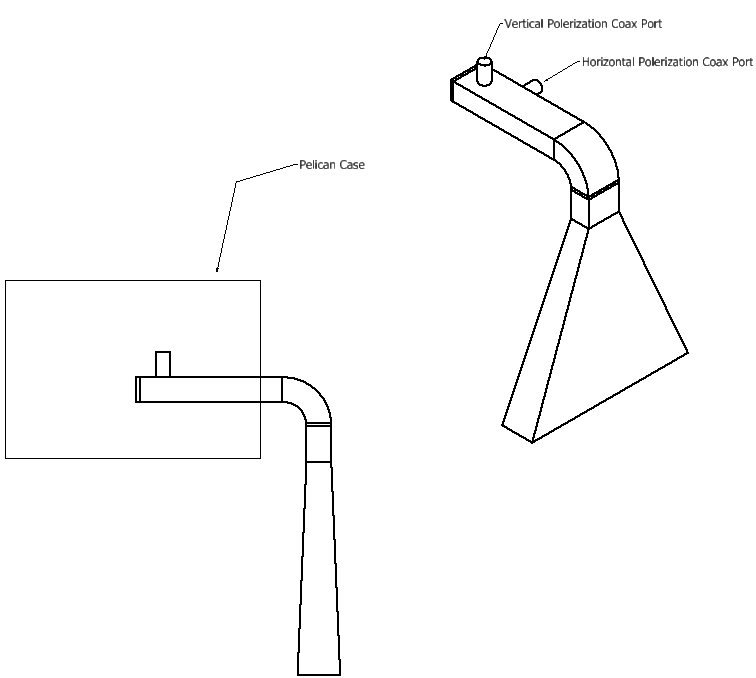
\includegraphics[width=0.5\linewidth]{Figures/rough_antenna.png}
	\label{fig:antenna}
	\caption{Horn antenna}
\end{figure}
The graph shown in figure \ref{fig:antenna_direction} shows the directivity of the antenna shown in figure
\ref{fig:antenna} (note that this is just an concept an not the final design). The directivity is high in 
the dimension where the antenna is large. This means that if we have a wide and thin antenna we are going to 
be scanning narrow bands along the ground. 
\begin{figure}
	\centering
	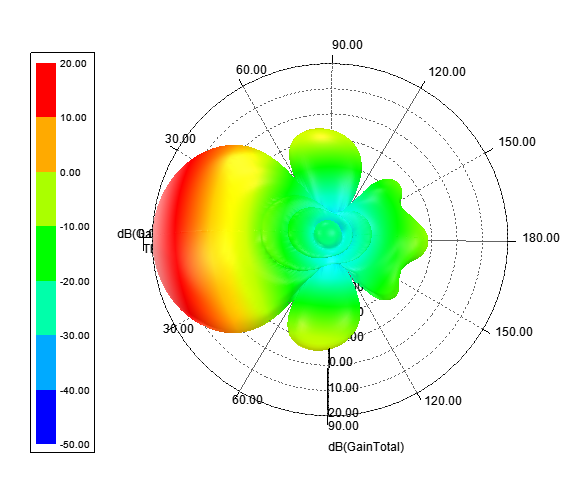
\includegraphics[width=0.5\linewidth]{Figures/antenna_gain.png}
	\label{fig:antenna_direction}
	\caption{Horn antenna directivity}
\end{figure}
One way of constructing the antenna is to have large copper sheets cut into shape then soldered together. While
this is fairly easy, it is imprecise and the resulting antenna is heavy. Another solution being investigated is
to 3D print the antenna, then chemically copper plate it. This will allow us to create more complicated geometry
and be much lighter then something made of solid copper. In house electroplating is being investigated for 
reduced cost, but the process in difficult and requires the development of procedures and techniques
\cite{bryancera2014}. Alternatively, a third party can be payed to electroplate our 3D print, though it would 
cost more.

\subsubsection{Radiometer Block Diagram}
David

\subsubsection{Band Selection}

Most soil moisture radiometers make use of L-band measurements (1-2 GHz), usually at or around 1.4 GHz. L-band measurements are ideal for soil moisture extraction for several reasons. First, the L-band is nearly transparent to vegetation, allowing for more accurate measurements. Second, the L-band penetrates up to a meter of soil, allowing deeper measurements which may indicate true groundwater content. Third, there is a reserved band for radio-astronomy at 1.4 GHz, reducing potential sources of interference. Lastly, RF components in the L-band have become increasingly cheap due to commercial uses for the L-Band such as WiFi and cellular networks. There is also a significant amount of literature and proven L-Band radiometer designs and models. The L-band however requires large antennas or complex measurement techniques to achieve directional measurements and build a map of soil moisture content. For example the radiometer aboard the SMOS satellite uses aperture synthesis and three large antennas ~1 meter in length to achieve a ground resolution of 35-50 km from a 755km orbit. \cite{Wigneron2010}. The SMAP mission uses a 6 meter dish antenna to achieve 40 km ground resolution from a 685 km orbit. \cite{entekhabi_njoku_oneill_spencer_jackson_entin_im_kellogg_2008}  For our radiometer, even a 30 cm dish only achieves a beam-width of 45 degrees at 1.4 GHz. Due to the spacial requirements of the CAN-SBX competition, even a 30 cm antenna might be too large. Thus, currently radiometers in the C-band (4-8 GHz) are being explored. C-band radiometers share some of the benefits of L-band radiometers. Components are still quite cheap due to the prevalence of WiFi and Bluetooth technology, there are some reserved radio-astronomy bands within the C-band, and there is some recent literature concerning soil moisture estimation from C-band radiometers. \cite{Description2000,jackson_gasiewski_oldak_klein_njoku_yevgrafov_christiani_bindlish_2002} However, the C-band does not penetrate the ground as far and can only accurately measure soil moisture to around 10-20 cm depth. Atmospheric microwave emissions are slightly stronger at the C-band, making it more difficult to accurately determine soil moisture content. The C-band is more greatly effected by ground vegetation type, water content in the ground vegetation canopy, and surface roughness effects, making accurate measurements more difficult or impossible. \cite{ulaby_fung_moore_1986} However, C-band radiometers offer much smaller antennas and much higher directionality and ground resolution. The same 30 cm parabolic dish antenna would achieve a 10 degree beam-width, allowing a ground resolution of 5 km at an altitude of 30 km. Both L-band and C-band options are currently being considered for the radiometer. A trade study table can be seen in table \ref{tab:band_trade}.

\begin{table}[!h]
	\centering
	\vspace{0.5cm}
	\renewcommand{\arraystretch}{1.3}
	\caption{Radiometer Band Trade Study. }
	\label{tab:band_trade}
	\begin{tabularx}{\textwidth}{lXll}
		\toprule
									& & L-Band & C-Band \\		
		\midrule
		Frequency					& &1-2 GHz&4-8 GHz \\ 
		Component Cost				& &Low&Moderate	 \\
		Antenna Size 				& &Large&Small	 \\
		Resolution 					& &Low Resolution&High Resolution 	\\ 
		Atmospheric Emission		& &Low&Moderate 					\\ 
		Effect of Vegetation		& &Low&Moderate						\\
		Effect of Surface Roughness	& &Low&Moderate						\\
		Ground Penetration			& &Up to 1 meter&10-20 cm			\\
	\end{tabularx}
\end{table}

\subsubsection{Soil Moisture Transfer Model}

To extract soil moisture content from radiometric data, a model of the received noise power must be formed. There are several parameters other than the soil moisture content that contribute to the total noise power measured by a radiometer. Surface roughness, surface temperature, presence and type of vegetation, atmospheric conditions, and antenna incidence angle all greatly effect the measured noise power and must be isolated to return an accurate soil moisture measurement. Isolating the ground moisture content is usually performed either by knowing tertiary information about the observed surface, or by making multiple measurements at different incidence angles, polarities, or frequencies. Our radiometer will measure the power spectral density over a wide band, but essentially only a single measurement will be made to reduce cost and complexity. Our radiometer will therefore have to rely on tertiary information such as open on-line datasets for earth ground cover, vegetation type, surface roughness, and surface temperature to eliminate several variables and obtain accurate measurements. Two methods are usually employed to solve for soil moisture content from the tertiary data and from the measured power spectral density.

\begin{enumerate}
\item Empirical models have been historically used to solve for soil moisture due to their computational simplicity. Several papers have performed experiments to determine models for various surface roughness's, vegetation types, and frequency ranges. These models can achieve accurate extraction of soil moisture content. Often though, these models are limited in scope due to the challenges in taking measurements over a a wide array of conditions. These models are also only suited for the specific instrument and measurements that the authors wish to make and are not applicable to a general case. Making our own empirical model is an option but would be time consuming and difficult.
\item Inverting a radiative transfer model allows the extraction of soil moisture content for any arbitrary radiometer, given that the parameters of the surface and atmosphere is well known at the desired frequency. This method is only as accurate as the ability to estimate the surface conditions and the applicability of the model to real world conditions. This method could introduce errors by ignoring some radiative effects or non-linearities that an empirical model might be able to account. Still, inverting a radiative transfer model allows for a more general solution that could by applied to any radiometric data. The zeroth order transfer function is the most basic form that has been used to extract soil moisture content and takes the form
%\boldblue{REMEMBER TO ADD THE IMAGE FROM ULABY OF THE ZRT MODEL AND THE EQUATION}
Since our radiometer is only measuring a single frequency and polarization, tertiary parameters must be determined from outside datasets. In an attempt to increase the accuracy of our radiometer system, the ZRT model will be derived as a function of the frequency and advanced parameter estimation techniques will be applied on the measure power spectral density. For example, a least squares parameter estimation technique could optimize the parameters of the ZRT model to fit the the measured power spectral density. It is expected that with this method alone, it will not be possible to eliminate every variable without resorting to tertiary datasets. However, it is expected that this could lead to more accurate estimation of soil moisture content.
\end{enumerate}

\subsubsection{Attitude Determination}

Depending on the achieved directionality of the antenna, it may be important to determine the actual attitude of the payload during the experiment to obtain an accurate map of the ground below. If a fairly non-directional antenna is chosen, then the attitude can safely be assumed to be always NADIR pointing. Sill, an IMU might still be included as modern MEMS IMU's are small, cheap and power efficient. Determining attitude from a 9-DoF accelerometer-gyroscope-magnetometer sensor is well explored in literature. Sensor fusion based on statistical methods or Kalman filtering is so commonplace that it could almost be considered trivial. A Kalman filter based on pendulum dynamics to model the balloon payload will be implemented to fuse the 9-DoF measurements and extract the current attitude. It is expected that this method will be more than accurate enough to account for minor attitude variations given the antennas expected beam-width. \cite{Vujicic2016} \cite{Estimation2017} \cite{Rhudy2017} \cite{Chow} \cite{Wan}

\begin{figure}[h!]
	\centering
	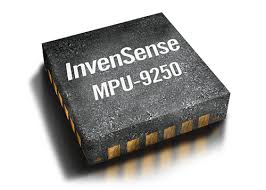
\includegraphics[width=.4\linewidth]{Figures/IMU.jpg}
	\caption{MPU9250 is a small modern low cost 9-DoF IMU}
	\label{fig:imu}
\end{figure}

\subsubsection{Experimental Procedures}
David
\subsubsection{Resources}
David
\subsubsection{Technical Risk Assessment}
Jacob
\begin{enumerate}
\item Human
\item Technical and Environmental
\end{enumerate}

\subsubsection{Team Structure}
There are currently two members on the CHARM team. Professor Bruce Burlton is acting as our faculty endorsement. We are also receiving a significant amount of help and guidance on the microwave design from professor Jim Wight.

\begin{enumerate}
\item Jacob Booth is responsible for data analysis, digital electronics design, attitude determination, the thermal reference control system, main controller software, and construction of the mechanical elements of the antenna .

\item David Bascelli is responsible for the radiometer RF section, antenna design, antenna construction, and digital signal processing of the power spectral density.

\end{enumerate}
\subsubsection{Project Time-line}
\subsubsection{Budget}
\subsubsection{Managerial Risk Assessment}


\section{Conclusion}

%-------------------------------------------------------------------------------
% REFERENCES
%-------------------------------------------------------------------------------
\newpage
\section{References}

\bibliography{radiometer}

\section{Appendix}


\end{document}
